\documentclass[../main.tex]{subfiles}

\begin{document}
In this chapter we give a brief explanation of the fundamental concepts involved in the
theory of homology, with special emphasis on those wich are relevant to persistent
homology. A standard treatment of homology can be found in chapter 2 of \cite{hatcher}.
Introductions to persistent homology in particular can be found at \cite{edelsbrunner08,
edelsbrunner12, edelsbrunner16}. 

\section{Introduction}
The standard elevator pitch for algebraic topology is as follows: classifying topological
objects is hard, whereas algebraic objects (groups, rings, etc) are better understood, so
algebraic topology provides tools to compute algebraic invariants from topological spaces,
which aids in their study. The natural setting for these ideas is category theory, so that
these ``tools'' become \emph{functors} from the category of topological spaces and
continuous maps, \( \Top \), to categories such as \( \Grp \), the category of groups and
group morphisms, or \( \Ab \), the category of abelian groups and their
morphisms\footnote{We will make some use of basic concepts from cateogry theory in this
chapter, a wonderful book on the topic is \cite{riehl}.}.

One of this tools are homology groups, which are the fundamental object of study in the
theory of homology. At the most abstract level, a theory of homology is a family of
functors from (some subcategory of) \( \Top \) to \( \Ab \) with a series of natural
transformations between them, subject to what are known as the \emph{Eilenberg-Steenrod
axioms}. For our purposes, however, such a general framework is not necessary, and we will
sismply describe one particular theory of homology, which is known as simplicial homology.
This theory is built in two steps. The first step has very much to do with the geometry of
the space we are considering and can be seen as a functor from the category of
\emph{simplicial complexes}, \( \Simp \), to the category of \emph{chain complexes of
abelian groups}, \( \Ch(\Ab) \), as explained in \cref{sec:geometric side}. This is
described in \cref{sec:geometric side}. Then there is a more algebraic step, in essence a
functor from \( \Ch(\Ab) \) to \( \Ab \), as seen in \cref{sec:algebraic side}. The hole
theory is then the composition of these two steps.

Finally, \cref{sec:persistence} gives an introduction to the ideas which underpin
persistent homology, which are the ones we will apply to the problem outlined in
\cref{ch:problem}. 

\section{The geometric side: simplices and simplicial complexes}\label{sec:geometric side}
As stated before, simplicial homology is restricted to simplicial complexes, which are,
roughly speaking, topological spaces assembled out of \emph{simplices}, which are the
generalisation of triangles and tetrahedra to higher dimensions. These spaces can be
described combinatorially, which makes them very useful for computation with datasets.
There are ways to generalise the theory to broader classes of spaces, such as singular
homology, but simplicial homology is sufficient for the analysis required. 

\subsection{Simplices}
As stated before, the basic building block of the spaces we will be dealing with are
simplicies. 
\begin{definition}[Simplex]\label{def:simplex}
	A simplex of dimension \( n \), or simply an \( n \)-simplex, generated by \( n+1 \)
	points of \( \R^d \) which do not lie in an affine subspace of dimension \( n
	\)\footnote{which means the ambient dimension \( d \) must be at least \( n \).}, is
	their convex hull, i.e. the smallest convex set which contains them.
\end{definition}
When a set of points generate a simplex they are called \emph{geometrically independent},
see \cref{fig:independence}. 

\begin{figure}[htb]
	\centering
	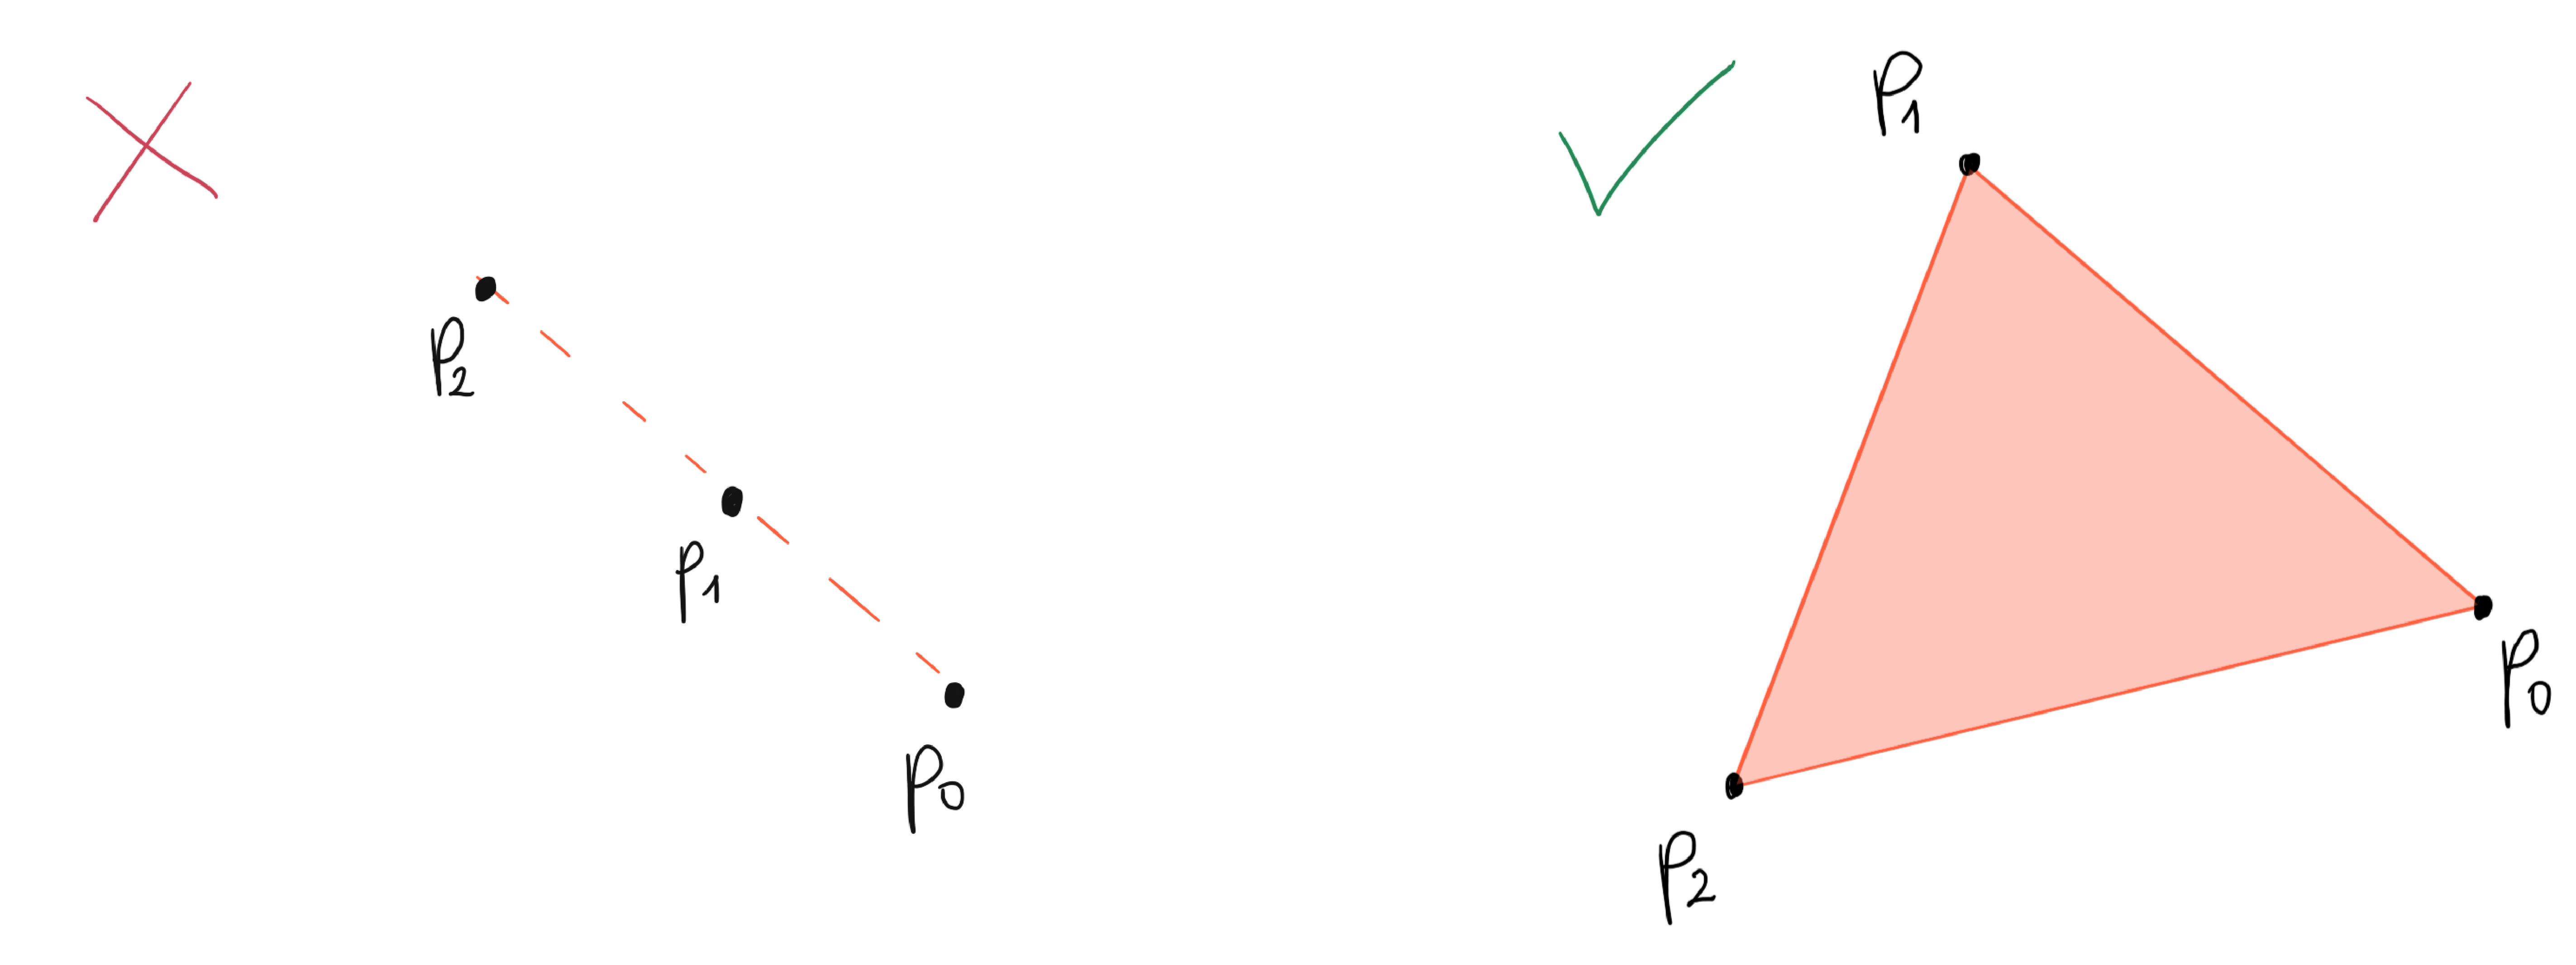
\includegraphics[width = 10cm]{independence}
	\caption{The three points on the left are not geometrically independent, whereas the
	three on the right are and so generate a 2-simplex.}
	\label{fig:independence}
\end{figure}

The \( n \)-simplex generated by the standard basis of \( \R^{n+1} \), \( e_0,
\dots, e_n \)\footnote{Because an \( n \)-simplex is generated by \( n+1 \)-points, it
will be convenient to number things starting at 0, as opposed to 1 as is more
common in mathematics.}, is called the \emph{standard \( n \)-simplex} and
written \( \Delta^n \). It can be shown that
\begin{equation*}
	\Delta^n = \set{(t_0, \dots, t_n) \in \R^{n+1} \mid \sum_{k = 0}^{n} t_k = 1, \forall k
	\leq n \colon t_k \geq 0}. 
\end{equation*}
The standard simplices provide a model for any other simplex. Indeed, if \( \phi \colon
\R^{n+1} \to \R^d \) is the linear map defined by \( \phi(e_k) = p_k \) for \( 0 \leq k
\leq n \) then \( \phi(\Delta^n) \) is precisely the simplex generated by \( p_0, \dots,
p_n \). \( (t_0, \dots, t_n) \) are called the \emph{barycentric coordinates} of the point
\( \phi(t_0, \dots, t_n) \). 

\subsubsection{Orientation}
For the purposes of homology, it is also important to keep track of the \emph{orientation} of a
simplex. We will use the idea of general simplices being the image of standard simplices
to model this situation
\begin{definition}[Ordered simplex]
	An \emph{ordered \( n \)-simplex} generated by \( p_0, \dots, p_n \in \R^d \) is a map
	\( \sigma \colon \Delta^n \to \R^d \) such that \( \sigma \) is the restriction to \(
	\Delta^n \) of the linear map \( \phi \colon \R^{n+1} \to \R^d \) given by \( \phi(e_k)
	= p_k \), provided \( p_0, \dots, p_k \) do indeed generate a simplex. 
\end{definition}
Observe that giving an ordering to the vertices of a simplex completely determines an
ordered simplex, thus we introduce the notation \( [p_0, \dots, p_n] \) for an ordered
simplex as defined above. 

Consider now the natural action of the symmetric group, \( \S_n \), on \( \R^n \) by
permuting the elements of the standard basis. Then, a reordering of an ordered \( n
\)-simplex \( \sigma \) is of the form \( \tau \circ \sigma \) for some \( \tau \in
\S_{n+1} \). Conversely, since the action of \( \S_n \) is free and transitive, for any
two ordered simplices with the same vertices,  \( \sigma_1 \) and \( \sigma_2 \) there
will always exist a unique permutation \( \tau \in \S_n \) such that
\begin{equation*}
	\sigma_1 = \tau \circ \sigma_2.
\end{equation*}
If \( \tau \) is even then \( \sigma_1 \) and \( \sigma_2 \) are said to have the same
orientation, whereas if \( \tau \) is odd then they are said to have opposite
orientations. This means in particular that there are only two possible orientations for
any simplex, which is consistent with the usual intuition for orientation. See
\cref{fig:orientation} for an example. 

\begin{figure}[htb]
	\centering
	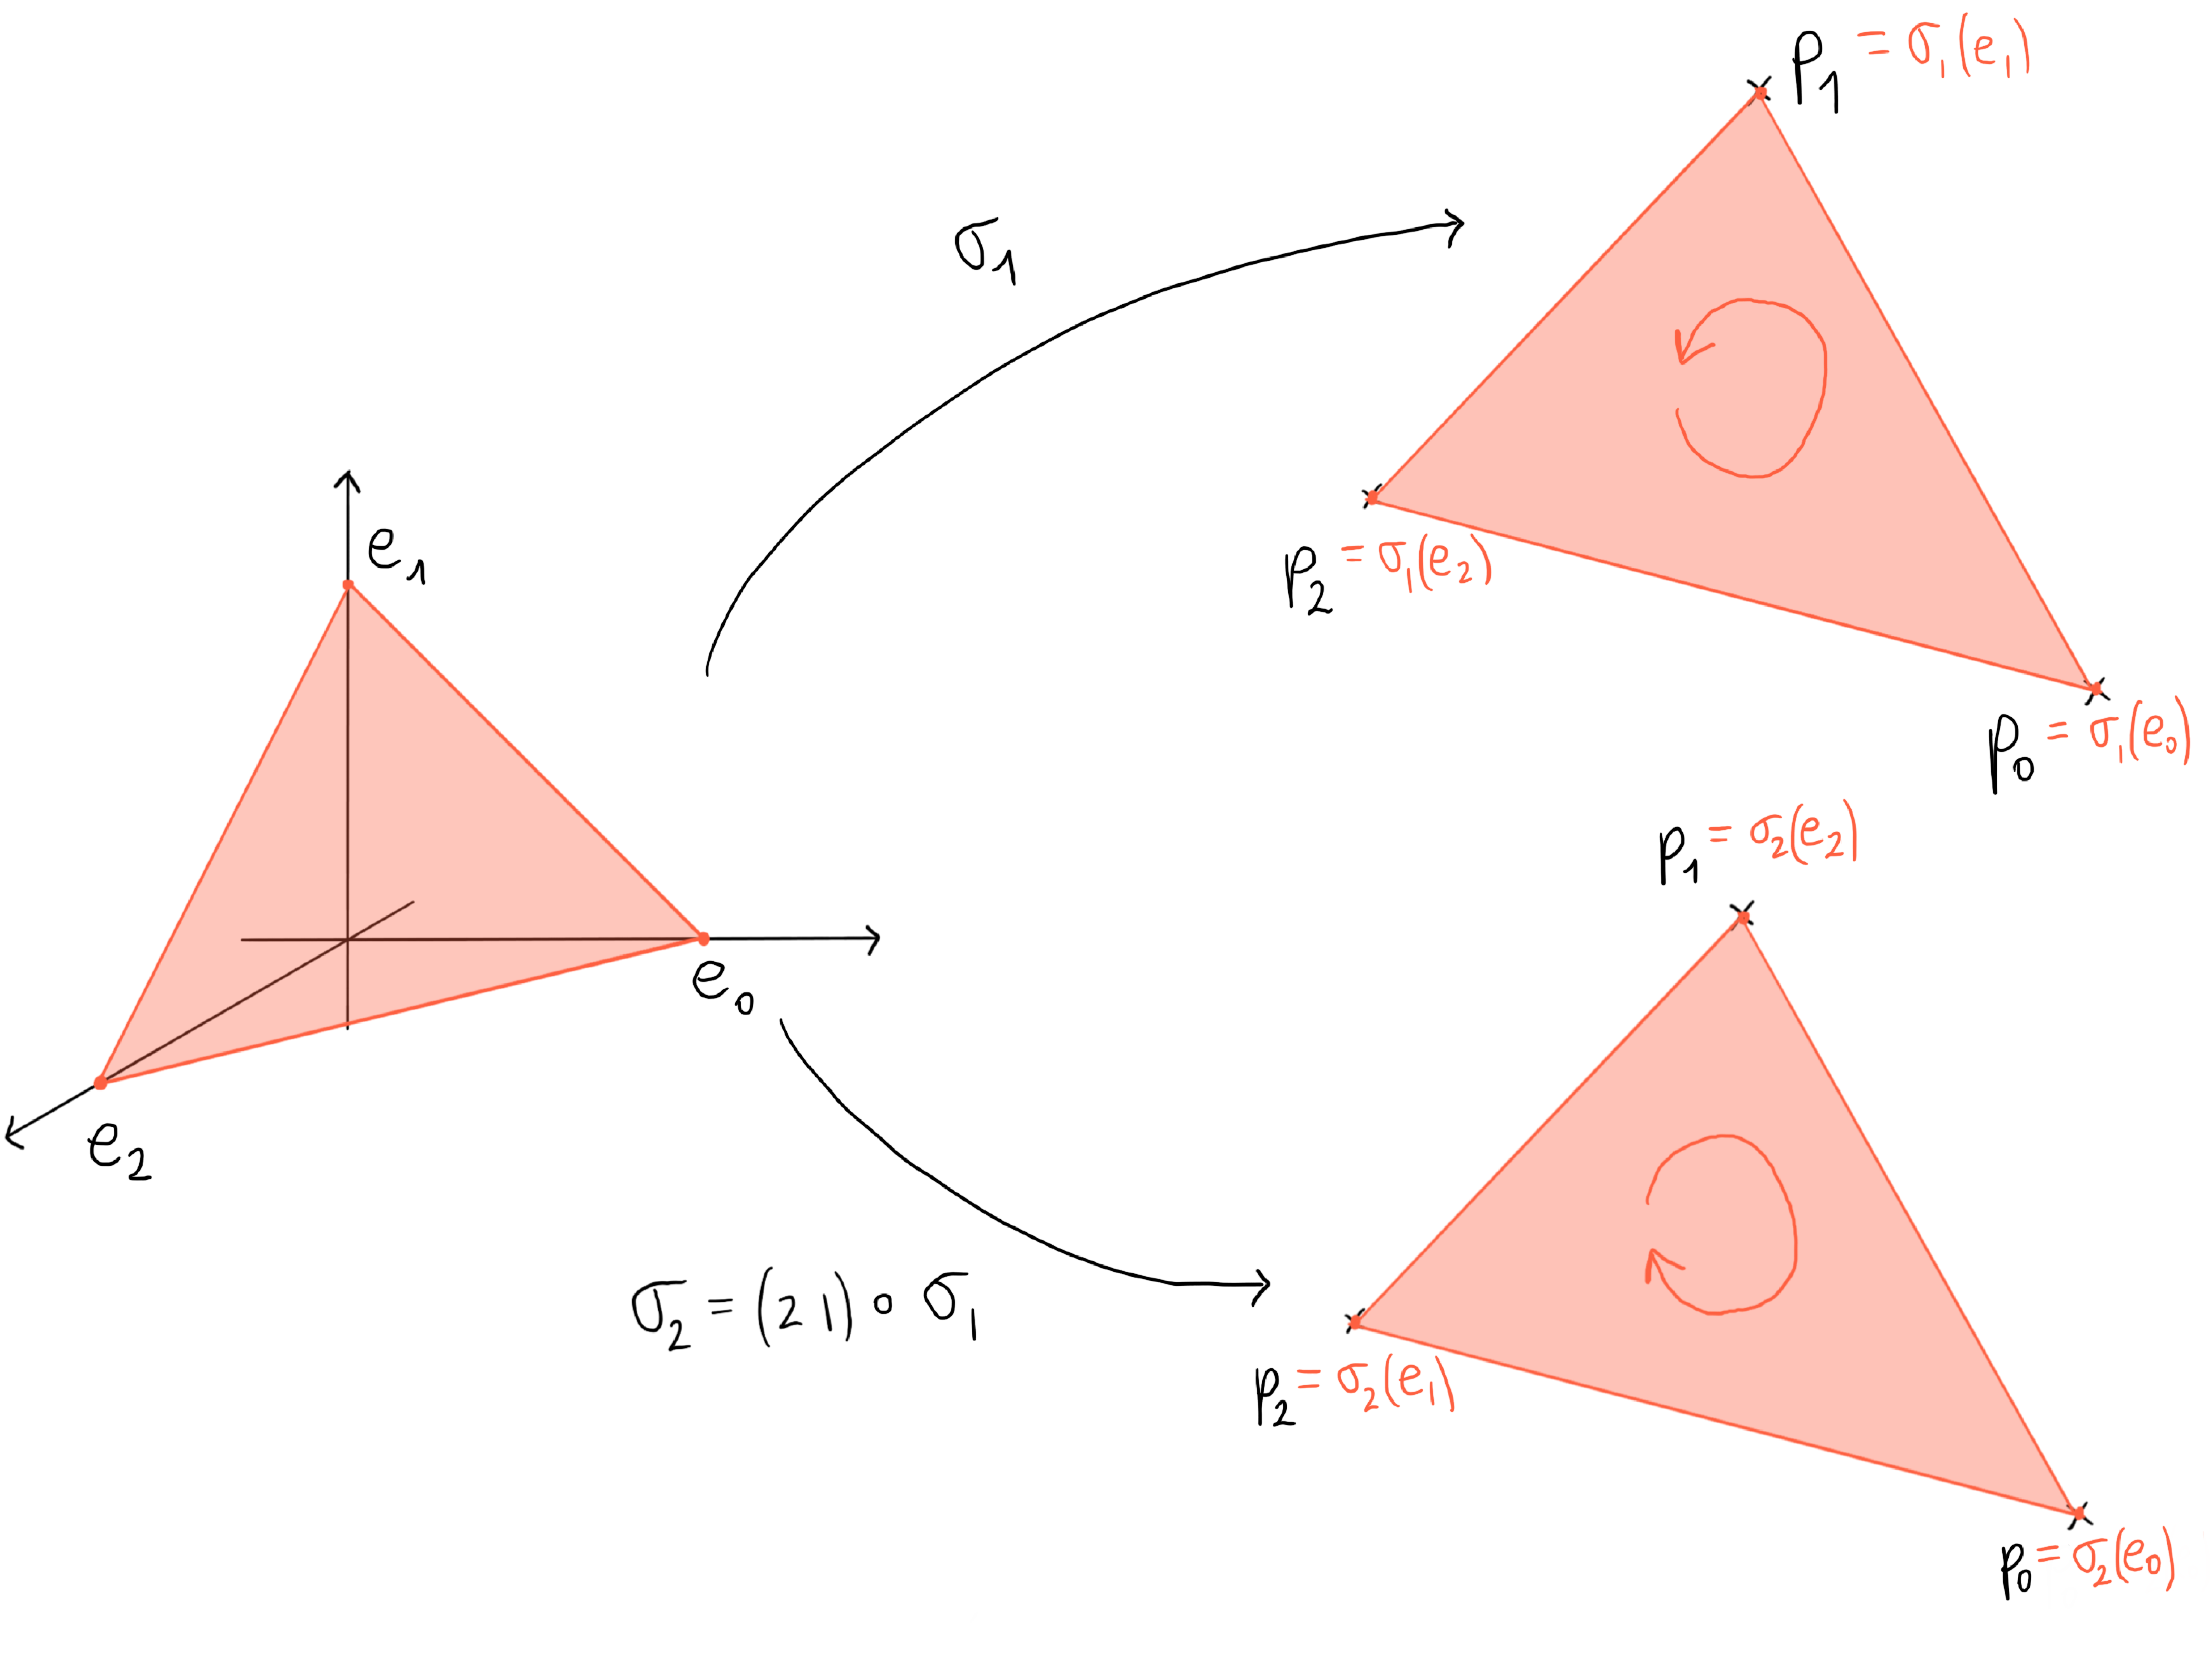
\includegraphics[width = 10cm]{orientation}
	\caption{Two different orderings of a 2-simplex with the same vertices that determine
	different orientations.}
	\label{fig:orientation}
\end{figure}

Given a simplex \( \sigma = [p_0, \dots, p_n] \), the \( n+1 \) possible simplices we get by
removing one of the generators ---i.e. \( [p_0, \dots, \hat{p}_k, \dots, p_n] \)--- are called the
\emph{faces} of \( \sigma \). Note that they are \( (n-1) \)-simplices in their own right
and they inherit an orientation from the orientation of \( \sigma \). 

\subsection{Simplicial complexes}
Simplicial complexes are spaces assembled out of properly glued together simplices, as the
following definition makes precise. 
\begin{definition}[Simplicial complex]\label{def:simplicial complex}
	A \emph{simplicial complex} \( K \) is a collection of simplices of \( \R^d \) such that 
	\begin{enumerate}[(i)]
		\item if \( \sigma \in K \) and \( \tau \in K \) is a face of \( \sigma \) then \(
			\tau \in K \),
		\item for any \( \sigma, \tau \in K \) then \( \sigma \cap \tau \in K \)\footnote{This
			is an abuse of notation since what is really meant is \( \sigma(\Delta^k) \cap
		\tau(\Delta^l) \).}. 
	\end{enumerate}
\end{definition}
The mental picture is that the simplices are only allowed to be glued along their faces. 

The simplices of \( K \) are often called its \emph{cells}, and we will write \( K_n \)
for collection of \( n \)-cells of \( K \). And the highest dimension of any of the cells
of \( K \) is the \emph{top dimension} of \( K \). 

A simplicial complex \( K \) determines a topological space, called its \emph{underlying
space}, which is the subset of \( \R^d \) determined by the union of (the images of ) all
of the cells of \( K \) equipped with the subspace topology, which we will write as \(
\abs{K} \). Pursuing the idea of realising more general topological spaces as underlying
spaces of some simplicial complex is what leads to singular homology. 

\subsection{Abstract simplicial complexes}
Notice that a simplex is always determined by its vertices, and vice versa, except for, of
course, whenever the vertices do not generate a simplex, in the sense of
\cref{def:simplex}. This requirement comes from thinking of simplices and simplicial
complexes as geometric objects. But if we don't think of them in this way, and simply
allow for any \( n+1 \) vertices to determine an \( n \)-simplex they become strictly
combinatorial objects. In this case, we also have to lift the second condition in the
definition of a simplicial complex, which was related to how the simplices are assembled
together as geometrical objects and therefore becomes meaningless in this new context. This more
general complexes are called \emph{abstract simplicial complexes} and are purely
combinatorial objects. From this viewpoint, an \( n \)-simplex is now an (ordered) set of
\( n+1 \) vertices, and its faces are just its subsets of \( n \) vertices. 
Ans so \cref{def:simplicial complex} is replaced by
\begin{definition}[Abstract simplicial complex]
	An \emph{abstract simplicial complex} \( K \) is any set closed under the relation of
	inclusion, i.e., if \( \sigma \in K \) then if \( \tau \subseteq K \), it must be the
	case that \( \tau \in K \).  
\end{definition}
For our purposes, we will assume that all of the simplices that make up a complex are
finite, that there is a maximum possible dimension  and that complexes are at most
countably infinite, thus avoiding problems related to size. This is not much of a
restriction since the main application are datasets which are finite. 

Notice that to specify a complex it suffices to exhibit its \emph{maximal simplices}, i.e.
those simplices which are not the face of any other simplex, or equivalently those which
are maximal with respect to inclusion\footnote{They are guaranteed to exist by requiring that the
dimensions of all simplices that make up the complex be bounded.}.

\subsection{Special complexes}
In the context of topological data analysis, one is often handed a bare point cloud and is
faced with the task of generating an appropriate simplicial complex. We now describe
various ways of doing this.  or the remainder of this section, \( X \) will denote a
finite subset of \( \R^d \), which models the raw point cloud we begin with. 

\subsubsection{Čech complex}
The \( \epsilon \)-Čech complex of \( X \), \( C_\epsilon(X) \), is determined by the
following prescription: \( \sigma \subseteq X \) is in \( C_\epsilon(X) \) if and only if
\begin{equation*} \bigcap_{p \in \sigma} B_\epsilon(p) \neq \emptyset \end{equation*}
where \( B_\epsilon(p) \) is the ball of radius \( \epsilon \) centered at \( p \). 

This does determine a simplicial complex, since if a certain set of vertices is such that
the intersection of all the \( \epsilon \)-balls centered at them is nonempty, then so
will the intersection of the corresponding balls for any subset be nonempty.

\subsubsection{Vietoris-Rips complex}
The prescription for the \( \epsilon \)-Vietoris-Rips
complex, \( V_\epsilon(X) \), is as follows: \( \sigma \subseteq X \) defines a simplex in
\( V_\epsilon(X) \) if and only if for every \( p, q \in \sigma \) 
\begin{equation*}
	B_\epsilon(p) \cap B_\epsilon(p) \neq \emptyset.
\end{equation*}
In other words, a set of points generate a simplex whenever each of them is at distance at
most \( 2\epsilon \)\footnote{Some texts use a slightly different convention such that the
vertices of a simplex in	\( V_\epsilon(X) \) are at distance at most \( \epsilon \) (rather
than \( 2\epsilon \)) from each other} from the rest. This also shows that the
Vietoris-Rips complex is indeed a complex.

Notice that the \( \epsilon \)-Čech complex is always a subcomplex\footnote{A subcomplex
of an abstract simplicial complex is a subset which is itself an abstract simplicial
complex.} of the \( \epsilon \)-Vietoris-Rips complex. Indeed, if \( [p_0, \dots, p_n] \) is a
simplex in \( C_\epsilon(X) \), then for any \( 0 \leq i,j \leq n \)
\begin{equation*}
	\emptyset \neq \bigcap_{k = 0}^n \subseteq B_\epsilon(p_i) \cap B_\epsilon(p_j)
\end{equation*}
so that \( [p_0, \dots, p_n] \) is also a simplex in \( V_\epsilon(X) \). The intuition is
that since the condition for a set of points to determine a simplex in the Vietoris-Rips
complex is weaker than for the Čech complex, the former will contain more simplices than
the latter.

\subsubsection{Clique complex} \label{sec:clique complex}
If the points of our cloud are the vertices of some graph, \( G \), we can use this
information to build the so-called clique complex, \( G(X) \), by declaring that \( \sigma
\subseteq X \) is a simplex of \( G(X) \) if and only if it is a clique, i.e. a
fully-connected subgraph of \( G \). This is indeed a complex since the graph generated by
any subset of vertices of a clique is itself a clique. The Vietoris-Rips complex is a
special case of this, since it is the clique complex of the graph obtained by declaring to
points of \( X \) adjacent when they are at distance at most \( 2\epsilon \).  The sort of
complex that will be used later is the clique complex of the \MKNN graph of the point
cloud. 

\section{The algebraic side: chain complexes and homology groups}\label{sec:algebraic
side}
So far we have dealt with the special kinds of spaces whose homologies we wish to compute.
We now turn to the actual task of computing. The main algebraic idea which requires
introduction is that of a chain complex, which, as opposed to the more restricted simplex,
plays an important role in the more algebraic aspects of any theory of homology, what is
aptly named hmological algebra. Out of the chain complexes we get the actual homology
groups, by a quotienting operation we will describe.

\subsection{Chain complexes}
\begin{definition}[Chain complex]
	A \emph{chain complex}\footnote{The word complex is being used for two different
		concepts: simplicial complexes and chain complexes. To avoid confusion we will adopt
		the convention that complex without qualifier refers to a simplicial complex whereas
	to refer to a chain complex we will always use both words.} (of abelian groups) is a
	family of abelian groups \( \set{C_n}_{n \in \N} \) together with a family of
	morphisms \( \partial_n \colon C_n \to C_{n-1} \) such that \( \partial_n \circ
	\partial_{n+1} \). We write \( (C_\ast, \partial_\ast) \) for the whole complex. 
\end{definition}
The elements of \( C_n \) are called \emph{\( n \)-chains}. The \( n \)-chains which lie
in \( \cyc{n} \) are the \emph{\( n \)-cycles}. And the chains in
\emph{\( \bound{n+1} \)} are called the \emph{\( n \)-boundaries}. It
follows from the definition of a chain complex that
\begin{equation*}
	\bound{n+1} \subseteq \cyc{n}
\end{equation*}
i.e. that every boundary is a cycle. This means the following definition makes sense.
\begin{definition}[Homology groups]
	The \emph{\( n \)-th homology group} of the chain complex \( (C_\ast, \partial_\ast) \)
	is the quotient
	\begin{equation*}
		H_n(C) \defeq \cyc{n} / \bound{n+1}.
	\end{equation*}
\end{definition}
Two elements which are the same when projected onto the homology group are called
\emph{homologous}. From the definition it is immediate to see that two chains are
homologous if they differ by a boundary, i.e. \( c_1 \) is homologous to \( c_2 \) if
there exists \( d \) such that \( c_1 = c_2 + \partial d \).

\subsection{Simplicial chain complexes}
The next step is building a chain complex out of the simplicial complexes we have built so
far and computing its homology groups. These will then be the homology goups of the
space. 

This chain complex is called, perhaps confusingly, a simplicial chain complex. Given a
simplicial complex \( K \), the corresponding simplicial chain complex, which we now
define, is written \( (C_\ast(K), \partial_\ast) \). We need each \( C_n(K) \) to be an
abelian group, so an easy way to achieve this is to define \( C_n(K) \) as the free
abelian group generated by the \( n \)-cells of \( K \). This is not quite it since we
want the orientation to play nicely with the group structure. We add the additional
condition that for any \( n \)-simplex \( \sigma \) and permutation \( \tau \in \S_n \),
\begin{equation*}
	\tau \circ \sigma = (-1)^\tau \sigma
\end{equation*}
where \( (-1)^\tau \) is the sign of \( \tau \). That is, if we reorder the vertices of \(
\sigma \) by an even permutation, so we don't change the orientation of \( \sigma \),
nothing changes. But if we reorder by an odd permutation, so that the orientation of \(
\sigma \) changes, a minus sign is picked up. 

In fact, once we have fixed an orientation for each of the cells of \( K \) we can
treat \( C_n(K) \) as a free group, so that an \( n \)-chain \( c \in C_n(K) \) is of the
form
\begin{equation*}
	\sum_{\sigma \in K_n} a_\sigma \sigma
\end{equation*}
for \( a_\sigma \in \Z \). 

Of course the other half of a chain complex are the boundary morphisms, which are defined
as follows
\begin{definition}[Boundary morphisms]
	We define, for \( n \geq 1 \), the morphisms
	\begin{equation*}
		\partial_n \colon C_n(K) \longto C_{n-1}(K)
	\end{equation*}
	by giving their action on a generator as
	\begin{equation*}
		\partial_n [p_0, \dots, p_n] \defeq \sum_{k = 0}^{n} (-1)^k [p_0, \dots, \hat p_k,
		\dots, p_n]
	\end{equation*}
	and extend them on any other chain by
	\begin{equation*}
		\partial_n\left(\sum_{\sigma \in K_n} a_\sigma \sigma\right) \defeq \sum_{\sigma \in K_n}
		a_\sigma \partial_n \sigma.
	\end{equation*}
\end{definition}
We need to show that all of this is indeed a chain complex, which is a consequence of the
following result.
\begin{lemma}
		For any \( n > 1 \), \( \partial_{n-1} \circ \partial_n = 0 \). 
\end{lemma}
\begin{proof}
	It suffices to show this on any generator, which is a simple calculation:
	\begin{align*}
		(\partial_{n-1} \circ \partial_n)[p_0, \dots, p_n] = {} & \partial_{n-1}\left(\sum_{k
		=		0}^{n}(-1)^k[p_0, \dots, \hat p_k, \dots, p_n]\right) \\
				= {} & \sum_{k = 0}^{n}(-1)^k	\partial_{n-1}[p_0, \dots, \hat	p_k, \dots, p_n] \\
				= {} & \sum_{k = 0}^{n}(-1)^k	\left(\sum_{l = 0}^{k - 1} (-1)^l [p_0, \dots, \hat	p_l, \dots, \hat p_k, \dots, p_n] \right. \\
						 & {} + \left. \sum_{l = k+1}^{n}(-1)^{l-1} [p_0, \dots, \hat p_k, \dots, \hat
						 p_l \dots, p_n]\right) \\
				= {} & \sum_{\mathclap{\substack{k = 0 \\ l < k}}}^n (-1)^k(-1)^l [p_0,	\dots,
				\hat p_l, \dots, \hat p_k, \dots, p_n] \\
						 & {} - \sum_{\mathclap{\substack{k = 0 \\ l > k}}}^n (-1)^k(-1)^l [p_0,
						 \dots, \hat p_k, \dots, \hat p_l, \dots, p_n] \\
				= {} & 0
	\end{align*}
	because both summands in the last line are the same. 
\end{proof}
Thus, if \( d \) is the top dimension of \( K \), we have the
simplicial chain complex
\begin{equation*}
	\begin{tikzcd}
		C_d(K) \arrow[r, "\partial_d"] & C_{d-1}(K) \arrow[r] & \cdots \arrow[r] & C_1(K)
		\arrow[r, "\partial_1"] & C_0(K) \arrow[r] & 0 
	\end{tikzcd}
\end{equation*}
We will drop the subscripts from the boundary morphisms whenever they can be deduced from
the context. 

\subsubsection{Interpretation}
The chain groups are related to the concatenation of loops in a general topological
space\footnote{As explained in \cite{hatcher}, the homology groups are in some sense the
abelianisation of the fundamental groups.} Indeed, the sum of two simplices can be
understood as their concatenation. Then, the boundary of a simplex is the sum of its
faces. Except not quite, because if we simply used the induced orientation for the faces
we would find that \( \partial_{n} \circ \partial_{n+1} \neq 0 \). Geometrically, what is
happening is that with the induced orientation, the faces don't ``go around nicely'', so
to say, and about half of them need their orientation flipped, which is what the
alternating sign accounts for. \cref{fig:boundary} shows this for the boundary of a
2-simplex.
\begin{figure}[htb]
	\centering
	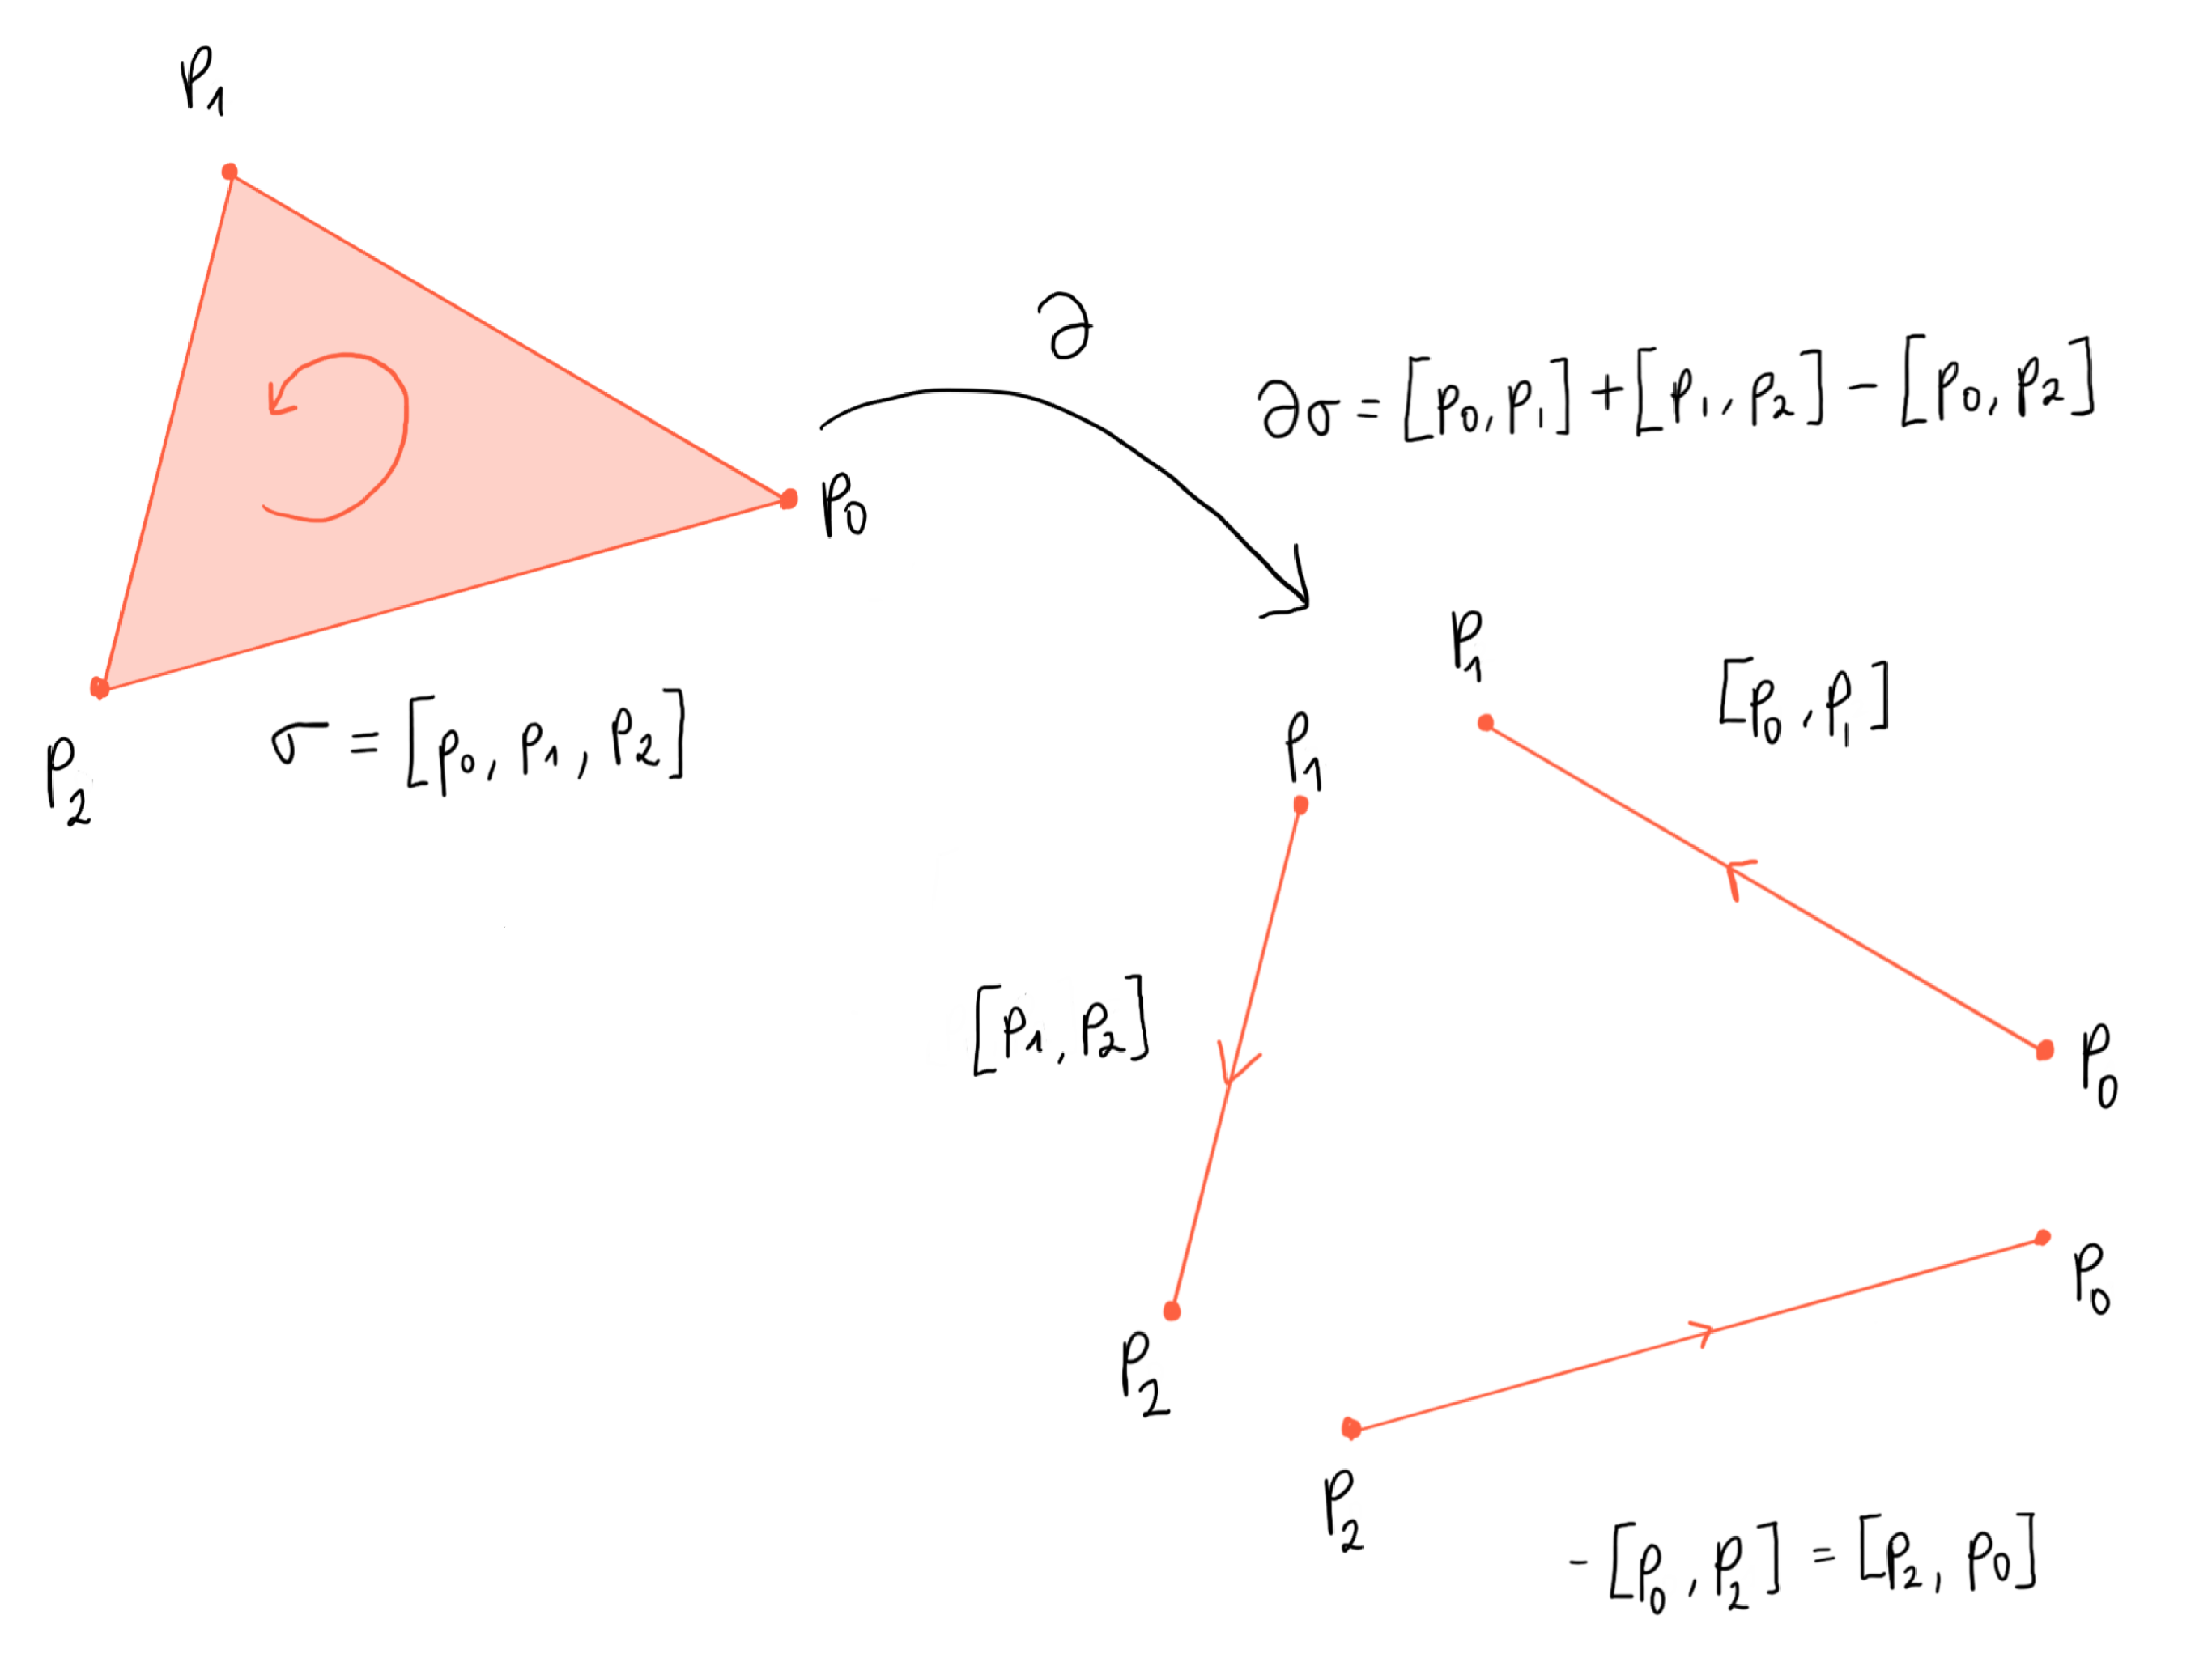
\includegraphics[width = 12cm]{boundary}
	\caption{This is a representation of the boundary of a 2-simplex. Notice that the face
		\( [p_0, p_2] \) is flipped, which results in the orientations of the boundary going
	around counterclockwise.}
	\label{fig:boundary}
\end{figure}
The more general interpretation of homology is discussed in \cref{sec:meaning}, however,
notice that the cycles and boundaries in a simplicial chain complex are cycles and
boundaries in the geometric sense and in fact this is the origin of the terminology. 

\subsubsection{Homology with different coefficients} \label{sec:different coefficients}
Instead of considering the free abelian groups generated by the cells, we could think
about the \( F \)-vector space they generate, for any field \( F \), subject to the
compatibility with orientation. Then we would get a chain complex of vector spaces. The
homology groups of this complex would be \( F \)-vector spaces. In this case, one defines
the \emph{Betti numbers} as
\begin{equation*}
	\beta_n(X, F) = \dim H_n(X, F)
\end{equation*}
where \( H_n(X, F) \) are the homology groups of the \( F \)-vector space chain
complex. 

The case of \( F = \F_2 \) will be of particular interest to us since the algorithm
implemented later computes homology with coefficients in \( \F_2 \). In this case we have
\begin{equation*}
	\tau \circ \sigma = (-1)^\tau \sigma = \sigma
\end{equation*}
so that this homology is orientation blind in some sense. In particular, the alternating
signs involved in the definition of \( \partial \) vanish. 

\section{The meaning of homology}\label{sec:meaning}
So we have described how to calculate, at least in principal, these homology groups, and
the claim at the beginning of this chapter was that they give us useful information about
the space at hand. the obvious question is then: what information exactly?

The first important point is to understand what homology \emph{cannot} tell us. It can be
shown that (singular) homology is invariant under homeomorphisms. But in fact it is also
invariant under homotopy equivalence, which is a much weaker relationship than
homeomorphism: a point is homotopically equivalent to \( \R^n \). This means it cannot be
used as a tool to classify spaces, at least not in the most general setting. 

The easiest homology group to interpret is \( H_0 \), since it can be shown that \(
\beta_0 \) is the number of connected components of the space. Higher homology groups
have to do with \( n \)-dimensional holes in the space.  Indeed, a cycle which is not the
boundary of anything indicates the presence of some sort of ``obstacle'' in the space.
What it means for two simplicial chains to be homologous is that they are both the
boundary of a higher dimensional chain, which is very similar, yet weaker, then the notion
of homotopy. Therefore, if there is a cycle which is not homologous to zero, it means it
cannot, very roughly speaking, be continuously deformed away.  instance, \( \beta_1 \) is
1 for \( S^1 \), which makes sense because \( S^1 \) is in some sense the prototypical
1-dimensional hole. For \( S^2 \), \( \beta_1 = 0 \) but \( \beta_2 = 1 \), reflecting the
fact that \( S^2 \) is ``hollow''. 

\section{The idea of persistence}\label{sec:persistence} 
So far we have seen various ways of extracting information related to the shape of our
data using homology. All of this ways, however, carry with them an ammount of arbitrary
choice. For example, both the Vietoris-Rips and Čech complexes depend on a scale parameter
\( \epsilon \), and the appropriate choice of \( \epsilon \) is generally not clear from
the data. The idea of persistent homology is to sidestep this problem altogether by
considering the homology of the data at every scale to determine which are the features
really reflect geometric aspects and which are byproducts of background noise. The first
will be, roughly speaking, those which are present at a large range of scales, i.e. those
which are \emph{persistent}. We now formalise these ideas.

\begin{definition}[Filtration]
	A \emph{filtration} is a family of simplicial complexes \( \set{K_i}_{i = 0}^n \)	such
	that \( K_i \) is a subcomplex of \( K_{i+1} \),
	\begin{equation*}
		K_0 \subseteq K_1 \subseteq \cdots \subseteq K_n
	\end{equation*}
	where we will mostly assume \( K_0 = \emptyset \). 
\end{definition}
The inclusions \( \iota_i^j \colon K_i \into K_j \), because of the
functoriality\footnote{Again, see \cite{riehl} for a detailed introduction to category
theory.} of homology, give rise to maps between the homology groups at different steps of
the filtration,
\begin{equation*}
	H_p(\iota_i^j) \colon H_p(K_i) \longto H_p(K_j)
\end{equation*}
which we will write as \( f_i^j \) for short. We say a certain class is \emph{born at \( i
\)} if it is not in the image of any \( f_k^i \) for any \( k \leq i \). And we say it
\emph{dies at \( j \)} if it is in the kernel of \( f_i^j \) but not of \( f_i^k \) for \(
k < j \). The difference \( j - i \) is called its \emph{persistence} or \emph{lifetime}. 

This is a reflection at the level of homology of how the shape of the complex changes at
every step of the filtration. See \cref{fig:filtration} for a detailed example.
\begin{figure}[htb]
	\centering
	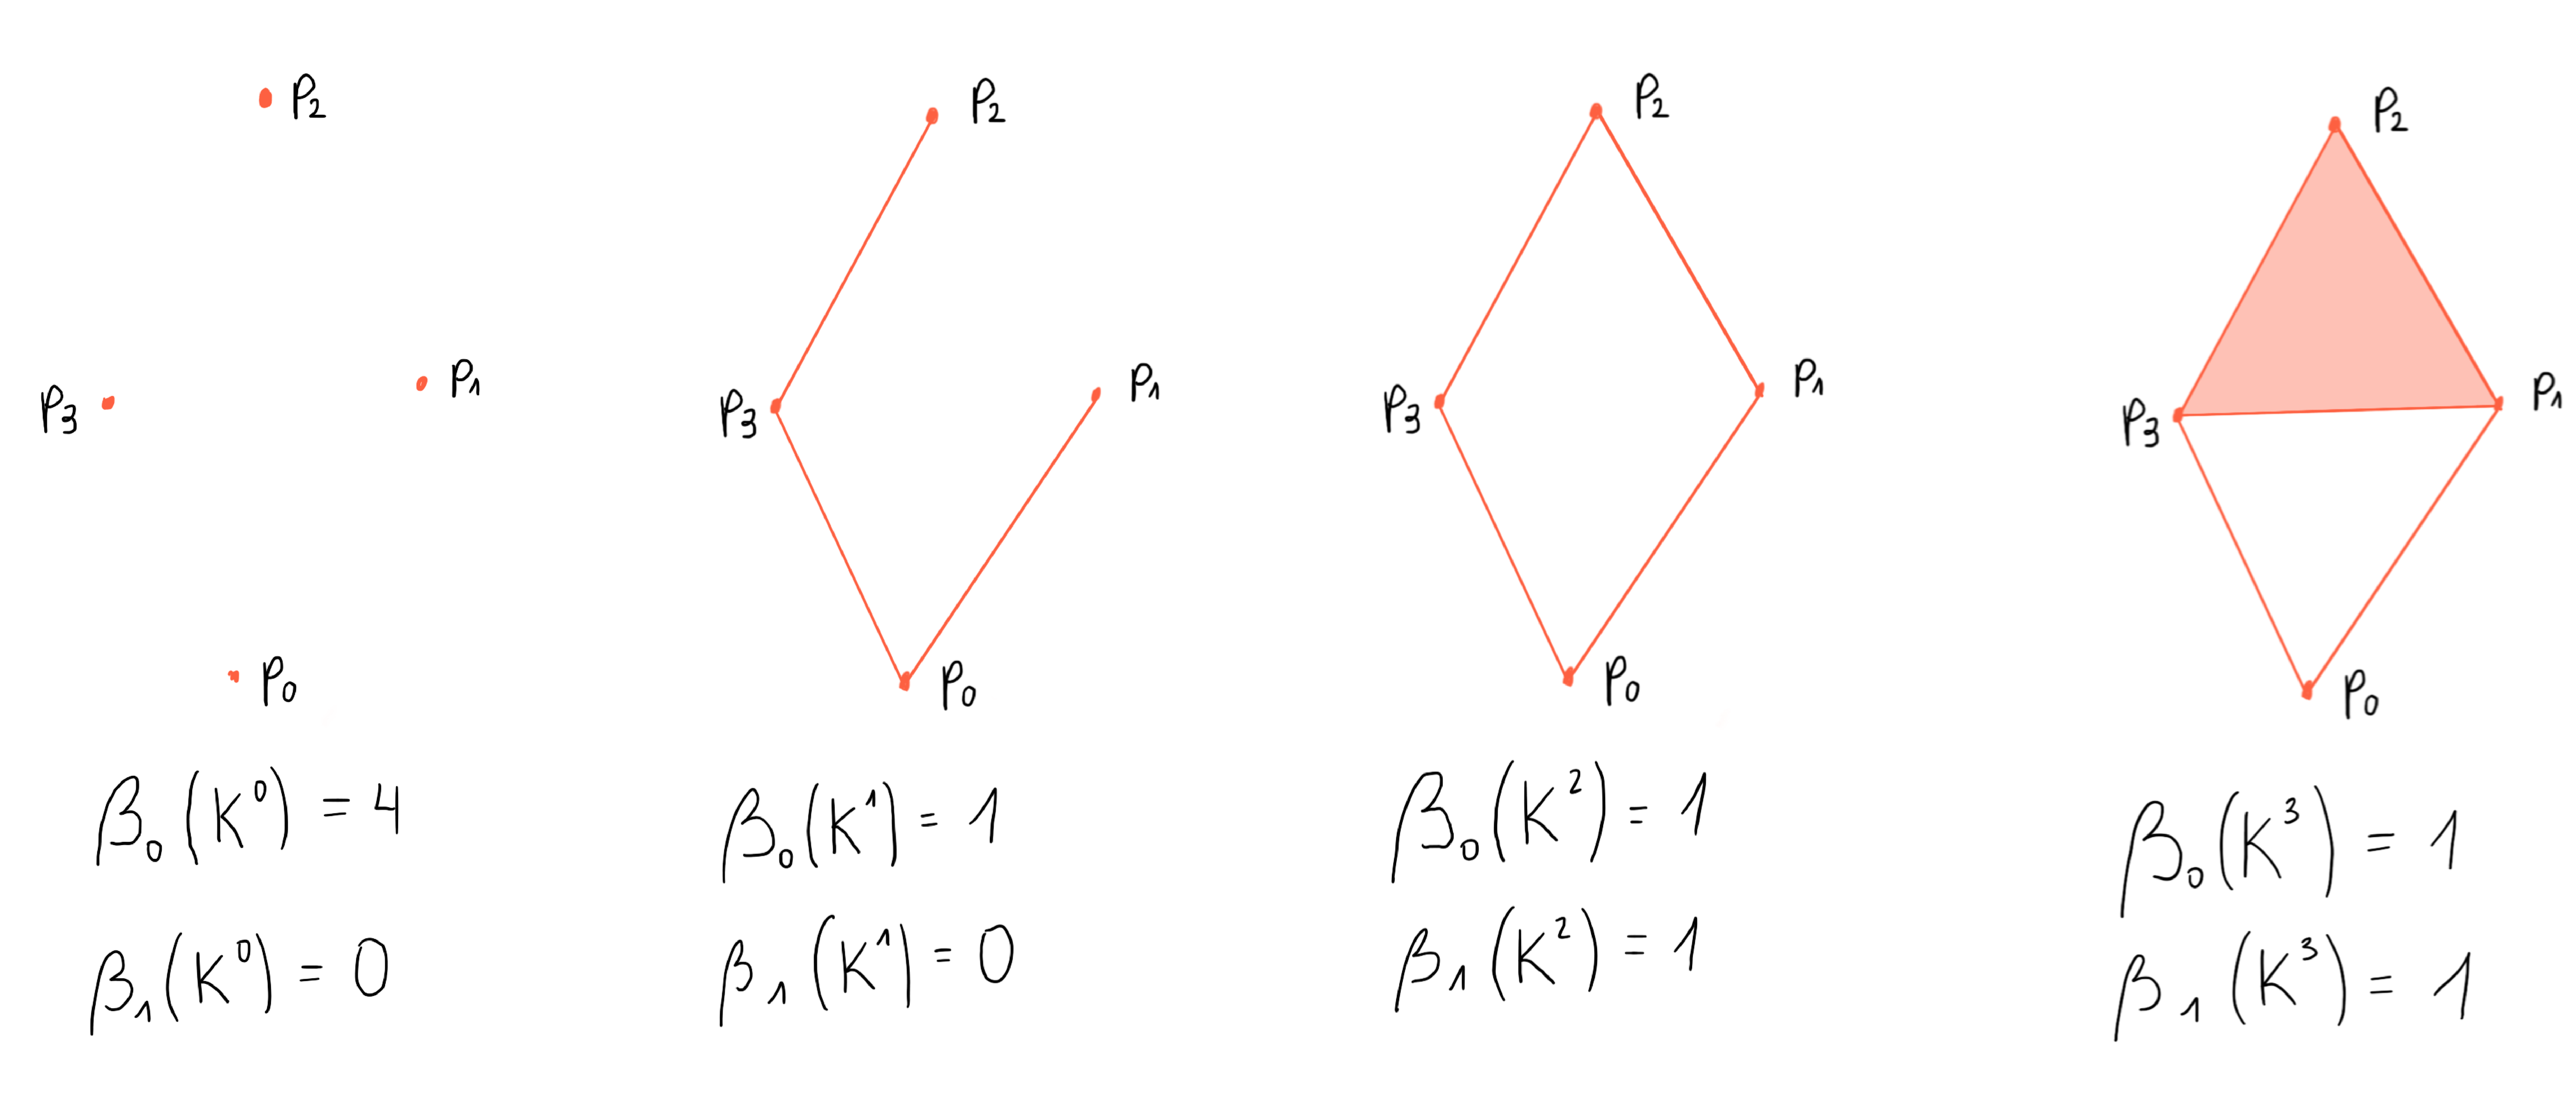
\includegraphics[width = 15cm]{filtration}
	\caption{Four different steps of a filtration and their first two Betti numbers. At the
		first step, the complex consist of four isolated points. At the next step, three
		1-simplices connect all the points but no combination of them is a cycle, so the dimension
		of \( H_1(K^1) \) is still 0. At the next step, the simplex \( [p_1,p_2] \) closes the
		cycle \( c = [p_0,p_1] + [p_1,p_2] + [p_2,p_3] + [p_3,p_0] \)	which is not the boundary of
		anything (there are no 2-simplices), and so the dimension of \( H_1(K^2) \) becomes 1.
		Finally, a 2-cell is born, but this is not sufficient to kill the class of \( c \).
	Indeed, \( f_2^3(c) = c = [p_0,p_1] + [p_1,p_3] + [p_3,p_0] + \partial[p_1,p_2,p_3] \).}
	\label{fig:filtration}
\end{figure}
The information that persistent homology is often encoded into what is known as a
\emph{barcode}, which is the birth and death of every element of the homology groups that
has lived at any of the steps of the filtration. 

\end{document}
